\documentclass{sig-alternate-ipsn13}

\begin{document}

\title{[This idea fails QAQ] Selfie Liberator - Touchless Camera Control by Using Trasformed Quadcopter}
%
% You need the command \numberofauthors to handle the 'placement
% and alignment' of the authors beneath the title.
%
% For aesthetic reasons, we recommend 'three authors at a time'
% i.e. three 'name/affiliation blocks' be placed beneath the title.
%
% NOTE: You are NOT restricted in how many 'rows' of
% "name/affiliations" may appear. We just ask that you restrict
% the number of 'columns' to three.
%
% Because of the available 'opening page real-estate'
% we ask you to refrain from putting more than six authors
% (two rows with three columns) beneath the article title.
% More than six makes the first-page appear very cluttered indeed.
%
% Use the \alignauthor commands to handle the names
% and affiliations for an 'aesthetic maximum' of six authors.
% Add names, affiliations, addresses for
% the seventh etc. author(s) as the argument for the
% \additionalauthors command.
% These 'additional authors' will be output/set for you
% without further effort on your part as the last section in
% the body of your article BEFORE References or any Appendices.

\numberofauthors{1} %  in this sample file, there are a *total*
% of EIGHT authors. SIX appear on the 'first-page' (for formatting
% reasons) and the remaining two appear in the \additionalauthors section.
%
\author{
% You can go ahead and credit any number of authors here,
% e.g. one 'row of three' or two rows (consisting of one row of three
% and a second row of one, two or three).
%
% The command \alignauthor (no curly braces needed) should
% precede each author name, affiliation/snail-mail address and
% e-mail address. Additionally, tag each line of
% affiliation/address with \affaddr, and tag the
% e-mail address with \email.
%
% 1st. author
\alignauthor
Chun-Yen Hsu\\
       % \titlenote{Dr.~Trovato insisted his name be first.}\\
       \affaddr{Carnegie Mellon University}\\
       \affaddr{94035 Mountain View}\\
       \affaddr{California, USA}\\
       \email{chunyenh@andrew.cmu.edu}
% Ben Trovato\titlenote{Dr.~Trovato insisted his name be first.}\\
%        \affaddr{Institute for Clarity in Documentation}\\
%        \affaddr{1932 Wallamaloo Lane}\\
%        \affaddr{Wallamaloo, New Zealand}\\
%        \email{trovato@corporation.com}
% % 2nd. author
% \alignauthor
% G.K.M. Tobin\titlenote{The secretary disavows
% any knowledge of this author's actions.}\\
%        \affaddr{Institute for Clarity in Documentation}\\
%        \affaddr{P.O. Box 1212}\\
%        \affaddr{Dublin, Ohio 43017-6221}\\
%        \email{webmaster@marysville-ohio.com}
% % 3rd. author
% \alignauthor Lars Th{\o}rv{\"a}ld\titlenote{This author is the
% one who did all the really hard work.}\\
%        \affaddr{The Th{\o}rv{\"a}ld Group}\\
%        \affaddr{1 Th{\o}rv{\"a}ld Circle}\\
%        \affaddr{Hekla, Iceland}\\
%        \email{larst@affiliation.org}
% \and  % use '\and' if you need 'another row' of author names
% % 4th. author
% \alignauthor Lawrence P. Leipuner\\
%        \affaddr{Brookhaven Laboratories}\\
%        \affaddr{Brookhaven National Lab}\\
%        \affaddr{P.O. Box 5000}\\
%        \email{lleipuner@researchlabs.org}
% % 5th. author
% \alignauthor Sean Fogarty\\
%        \affaddr{NASA Ames Research Center}\\
%        \affaddr{Moffett Field}\\
%        \affaddr{California 94035}\\
%        \email{fogartys@amesres.org}
% % 6th. author
% \alignauthor Charles Palmer\\
%        \affaddr{Palmer Research Laboratories}\\
%        \affaddr{8600 Datapoint Drive}\\
%        \affaddr{San Antonio, Texas 78229}\\
       % \email{cpalmer@prl.com}
}
% There's nothing stopping you putting the seventh, eighth, etc.
% author on the opening page (as the 'third row') but we ask,
% for aesthetic reasons that you place these 'additional authors'
% in the \additional authors block, viz.
\additionalauthors{Additional authors: John Smith (The Th{\o}rv{\"a}ld Group,
email: {\texttt{jsmith@affiliation.org}}) and Julius P.~Kumquat
(The Kumquat Consortium, email: {\texttt{jpkumquat@consortium.net}}).}
\date{30 July 1999}
% Just remember to make sure that the TOTAL number of authors
% is the number that will appear on the first page PLUS the
% number that will appear in the \additionalauthors section.

\maketitle
\begin{abstract}

We design Selfie Liberator, a wearable quadcopter that can control camera direction by hand gesture and fastens on the wrist with no personal carry burden to provide user a better experience while taking selfie.

\end{abstract}

% problem:
% 1. selfie stick
%        1.1 bad technique
%        1.2 bring it 
% 2. front camera
%        1.1 bad resolution
% Both: cant not make bigger distance       

% connected by bluebooth


\section{Introduction}

With today's demand of selfie, several products and innovation ideas provide easier way to take selfie. For example, most of the smartphones and tablets have front camera, or using selfie stick which provide users an simple way to take selfie. 
% Another example such as selfie stick can also give user a better photograph after taking the selfie. 
However, 
% there are still several points that we can improve to approach better user experience. 
Because of the cost consideration, smartphone manufacturers seldom provides great resolution camera for the phone's front camera. The front camera would have less resolution and worse technique than the back camera in most cases. In addition, camera on the phone can not provide a broader view while taking selfie by ourself because of hand length limitation. Selfie stick can solve the problem of hand length limitation. Nevertheless, 
% it still results in several problems. For instance, 
users would not be willing to bring one more thing, such as a stick, just because of taking selfie. 

We present Selfie Liberator (Figure \ref{fig:demo1}) which provides a wearable camera by using the idea of quadcopter. We transfered the quadcopter to four arms that can be twisted to fasten on user's wrist. A high resolution camera is embedded in Selfie Liberator and can track user's gesture by computer vision technique. Whenever using it, user can just flick it off from user's wrist and let it fly away by itself. In addition, Selfie Liberator will fly back automatically after each selfie taken. Selfie Liberator not only solve the problem of the limitation of hand length 
% which can not take photograph with enough broad view 
but also provide user easier way to bring 
% which can just fasten on user's wrist 
with no additional personal carry required.
After analyzing our 22 user cases, results show that Selfie Liberator can significantly provide better user experience while taking selfie and produce better photograph comparing to selfie stick and smartphone front camera.


% \begin{figure}
% \centering
% 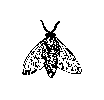
\epsfig{file=fly.eps}
% \caption{A sample black and white graphic (.eps format).}
% \label{fig:example}
% \end{figure}

\begin{figure}
  \centering
  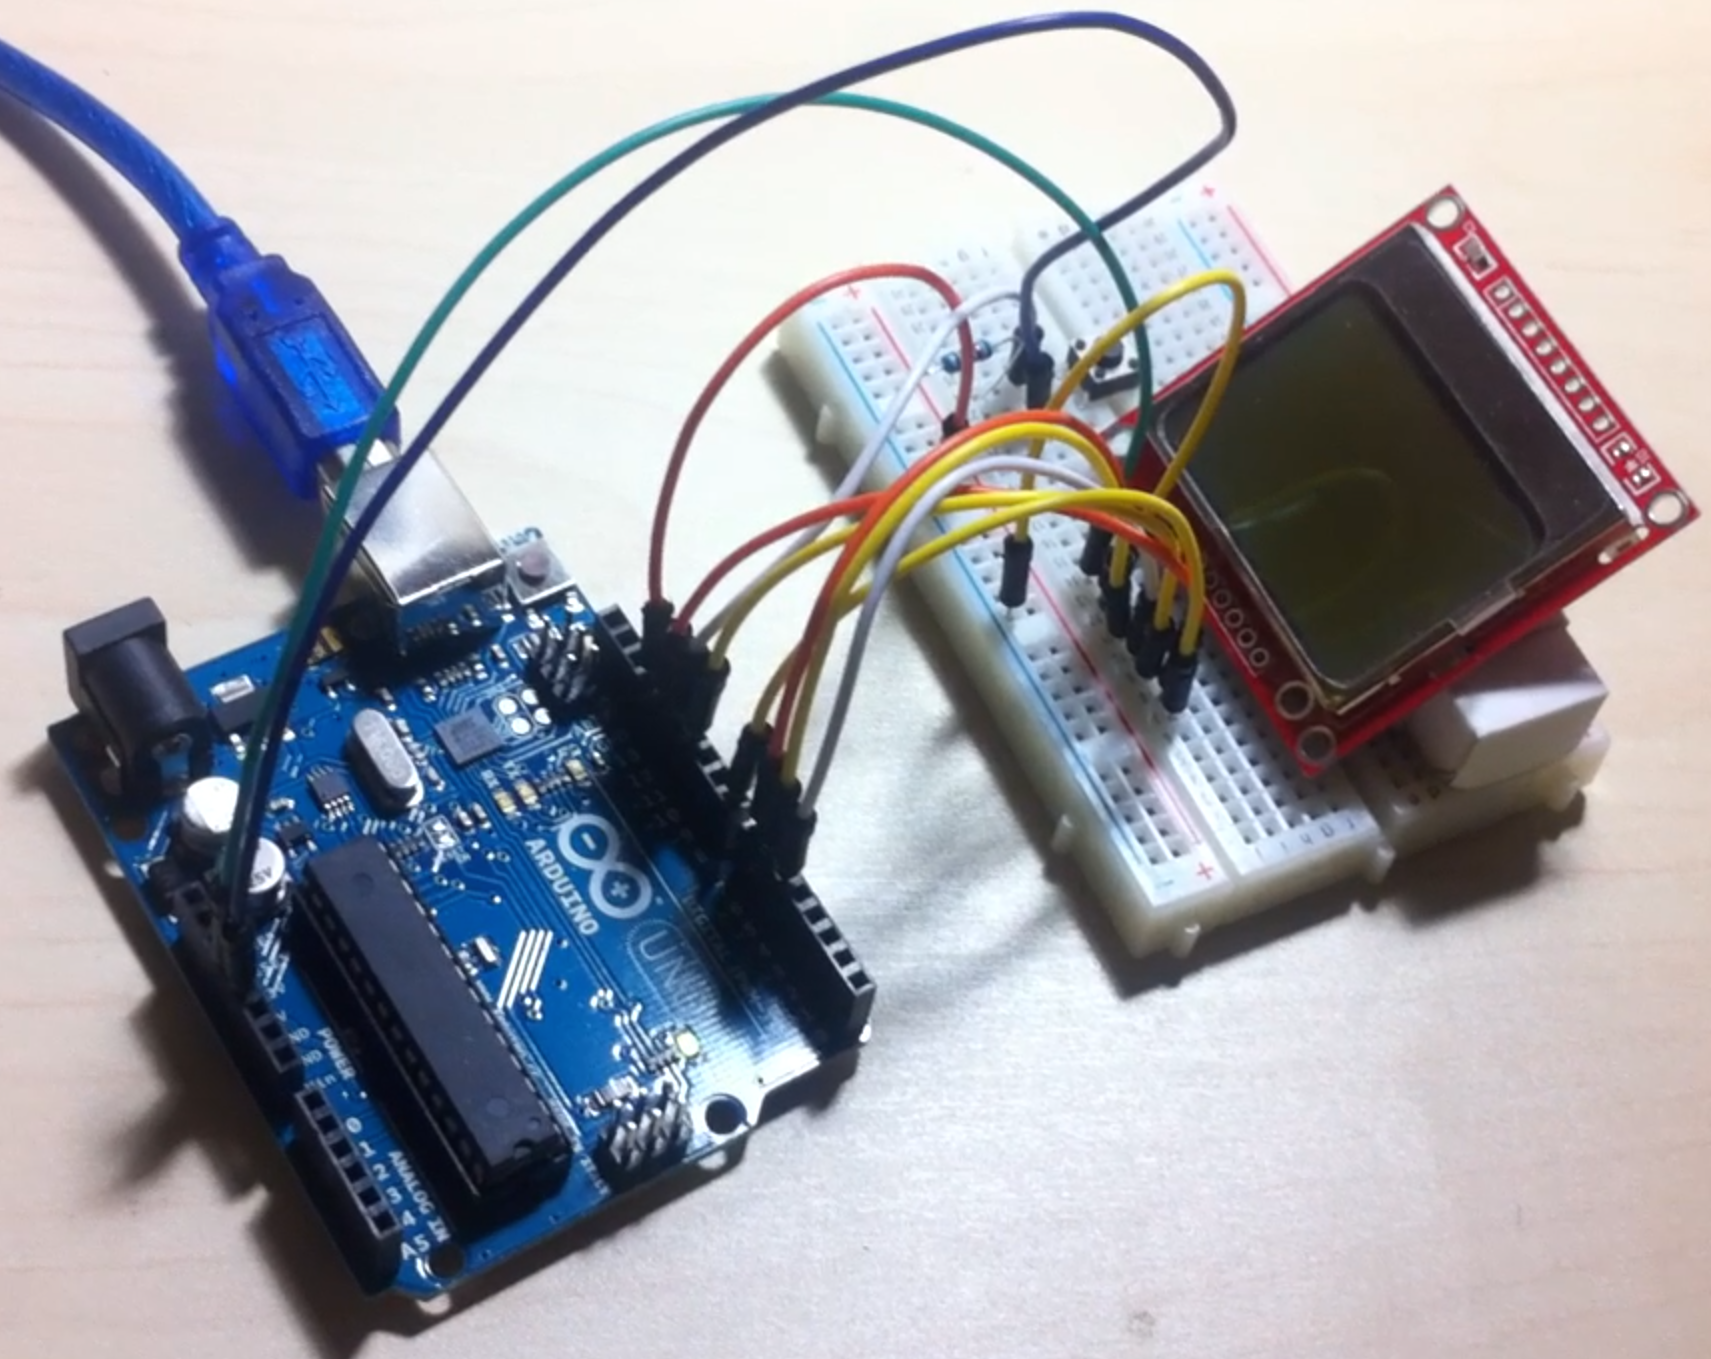
\includegraphics[width=0.8\linewidth]{Figures/demo1.pdf}
  \caption{Selfie Liberator, twist to fasten on human wrist with no personal carry burden }
  \label{fig:demo1}
\end{figure}

\section{Related Work}
Mueller's quadcopter work\cite{cite1} focuses on creating robotic systems to support exertion experiences, which also has the same idea with our design. Selfie Liberator is also used at outdoor activity and provide infinite quadcopter usage possibility for future research work.

% Jogging is a popular exertion activity. The abundance of jogging apps suggests to us that joggers can appreciate the opportunity for technology to support the jogging experience. We want to take this investigation a step further by exploring if, and how, robotic systems can support the jogging experience. We designed and built a flying robotic system, a quadcopter, as a jogging companion and studied its use with 13 individual joggers. By analyzing their experiences, we derived three design dimensions that describe a design space for flying robotic jogging companions: Perceived Control, Focus and Bodily Interaction. Additionally, we articulate a series of design tactics, described by these dimensions, to guide the design of future systems. With this work we hope to inspire and guide designers interested in creating robotic systems to support exertion experiences.

% \section{Evaluation and Limitation}
% Evaluation
% For example, user can not add the time by using light sensor in a dark room. This approach is the next challenge we are going to face.

\section{Conclusions}
Selfie Liberator provides not only a convenient way for user easier to bring it by fastening on user's wrist but also a better method to capture greater and broader photograph by hand gesture control. With Selfie Liberator, we don't need to ask others for help anymore if we pursue a great photograph and all of us should in it. It is no doubt that Selfie Liberator provides a better solution and indeed solve our life problem. 

%ACKNOWLEDGMENTS are optional
% \section*{Acknowledgments}
% Acknowledgement goes here.

%
% The following two commands are all you need in the
% initial runs of your .tex file to
% produce the bibliography for the citations in your paper.
\bibliographystyle{abbrv}
\bibliography{sigproc}  % sigproc.bib is the name of the Bibliography in this case
% You must have a proper ".bib" file
%  and remember to run:
% latex bibtex latex latex
% to resolve all references
%
% ACM needs 'a single self-contained file'!
%
%APPENDICES are optional
%\balancecolumns
% \appendix
%Appendix A

% Appendix goes here.

% That's all folks!
\end{document}
